\begin{myprop}
	\begin{itemize}
		\item Dans un triangle la longueur d'un coté est \\ \hspace*{6cm} des longueurs des deux autres côtés.
		
	\end{itemize}
	
\end{myprop}

\begin{mymeth}
	Pour vérifier qu'un \hspace*{6cm}, on vérifie que la longueur du plus grand côté  est inférieure à la somme des deux autres.
\end{mymeth}

\begin{myexs}
	\begin{multicols}{2}
		\begin{itemize}
			\item Dans le triangle ABC ci-contre on a %$AB < AC + CB.$
			\item Un triangle de cotés 8 cm, 5 cm et 6 cm est %constructible (8 < 11)
			
			\item Le triangle $DEF$, tel que $DE = 7$ cm, $DF = 3$ cm et $FE = 4$ cm est  %plat, les points sont alignés ($4 + 3 = 7$). 
			\vspace*{1cm}
			\item Un triangle de coté 10 cm, 4 cm et 5 cm %n'est pas constructible ($10 > 4 + 5$).
		\end{itemize}
		
		
		\begin{center}
			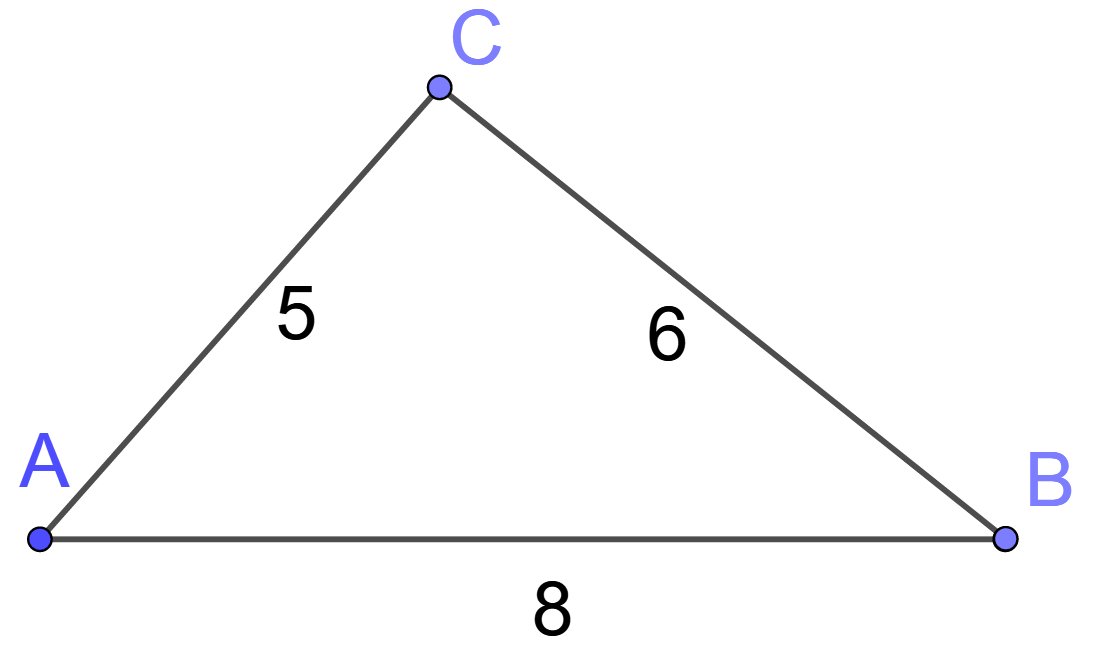
\includegraphics[scale=0.25]{triangle1}
		
		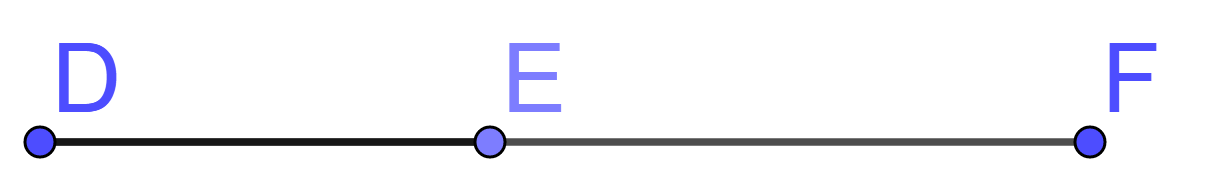
\includegraphics[scale=0.2]{triangle2}
		\end{center}
	\end{multicols}
\end{myexs}

